\paragraph{\trMatchingCycle{}重访。}\label{sub:matching-cycles-revisited}
取\cref{thm:tw-directed-quasiequiv}中那个\trQuasiequivalence{}的一个逆，并把它记作
\begin{equation*}
\mathscr{G}\colon Tw\scr{F}(\pi)\longrightarrow Tw\scr{F}^{\rightarrow}(\boldsymbol{V}^{\#}_{\boldsymbol{\gamma}}).
\end{equation*}
我们的第一个观察是：可以确定每个 (B) 型\trEquivariant\trBrane{}在 $\mathscr{G}$ 之下的像。按构造，对定义 $\mathscr{G}$ 时所用的那个具体的基，我们有
\begin{equation*}
\mathscr{G}(\widetilde{\Delta}^{\#}_{\gamma_j})=V^{\#}_{\gamma_j},
\end{equation*}
其中右边是看成 $\scr{F}^{\rightarrow}(\boldsymbol{V}^{\#}_{\boldsymbol{\gamma}})$ 自身的第 $j$ 个\trObject{}的那个\trVanishingCycle。现在考虑任意一个集合 $\boldsymbol{\delta}$ 及其第 $k$ 个初等\trHurwitz{}移动 $\boldsymbol{\rho}=\mathscr{L}_k\boldsymbol{\delta}$。于是，利用\cref{thm:twist-functorial-isomorphism}与\cref{thm:hurwitz-pi-twist-isomorphic}，我们发现
\begin{equation}\label{eq:g-hurwitz-images}
\mathscr{G}(\widetilde{\Delta}^{\#}_{\rho_j})\cong
\begin{cases}
\mathscr{G}(\widetilde{\Delta}^{\#}_{\delta_j}) & \text{对于 } j\neq k,k+1,\\
\mathscr{G}(\widetilde{\Delta}^{\#}_{\delta_k}) & \text{对于 } j=k+1,\\
T_{\mathscr{G}(\widetilde{\Delta}^{\#}_{\delta_k})}\mathscr{G}(\widetilde{\Delta}^{\#}_{\delta_{k+1}}) & \text{对于 } j=k.
\end{cases}
\end{equation}
其中 $\cong$ 是在 $D\scr{F}^{\rightarrow}(\boldsymbol{V}^{\#}_{\boldsymbol{\gamma}})$ 中取的，而且事实上可能只在相差\trTranslation{}的意义下成立（除非额外费心去追踪正确的\trGrading{}，这一点我们不作坚持）。通过代入，可以对逆\trHurwitz{}移动 $\boldsymbol{\sigma}=\mathscr{L}_k^{-1}\boldsymbol{\delta}$ 建立一个类似的公式，即
\begin{equation*}
\mathscr{G}(\widetilde{\Delta}^{\#}_{\sigma_j})\cong
\begin{cases}
\mathscr{G}(\widetilde{\Delta}^{\#}_{\delta_j}) & \text{对于 } j\neq k,k+1,\\
\mathscr{G}(\widetilde{\Delta}^{\#}_{\delta_{k+1}}) & \text{对于 } j=k,\\
T^{\vee}_{\mathscr{G}(\widetilde{\Delta}^{\#}_{\delta_{k+1}})}\bigl(\mathscr{G}(\widetilde{\Delta}^{\#}_{\delta_k})\bigr) & \text{对于 } j=k+1.
\end{cases}
\end{equation*}
每条\trVanishingPath{}都是某个\trDistinguishedBasis{}的一部分，这就完成了我们对第一步的解释。
接下来，设 $\mu$ 是一条\trMatchingPath，它相对于 $\boldsymbol{\delta}$ 的位置如\cref{fig:matching-path-position}所示。由\cref{thm:matching-delta-hf-sphere}，$D\scr{F}(\pi)$ 中从 $\widetilde{\Delta}^{\#}_{\delta_k}$ 到 $\widetilde{\Delta}^{\#}_{\delta_{k+1}}$ 的\trMorphism{}空间有两个\trGenerator，它们所在的\trDegree{}相差 $n$。至于确切的绝对\trDegree，则取决于诸\trGrading{}的选取，我们将对这些\trGrading{}作\trTranslation，直到两个\trDegree{}变成 $0$ 与 $n$ 为止。
\begin{figure}[htbp]
\centering
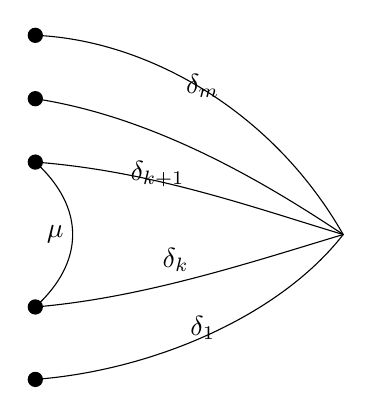
\begin{tikzpicture}[line cap=round,line join=round,scale=1.15]
\fill (0,3.8) circle (2.4pt);
\fill (0,3.1) circle (2.4pt);
\fill (0,2.4) circle (2.4pt);
\fill (0,0.8) circle (2.4pt);
\fill (0,0) circle (2.4pt);
\draw (0,3.8) .. controls (1.2,3.75) and (2.6,3.0) .. (3.4,1.6);
\node[anchor=south] at (1.85,3.0) {$\delta_m$};
\draw (0,3.1) .. controls (1.3,2.9) and (2.5,2.2) .. (3.4,1.6);
\draw (0,2.4) .. controls (1.3,2.3) and (2.4,1.9) .. (3.4,1.6);
\node[anchor=south] at (1.35,2.02) {$\delta_{k+1}$};
\draw (0,0.8) .. controls (1.2,0.9) and (2.4,1.3) .. (3.4,1.6);
\node[anchor=south] at (1.55,1.08) {$\delta_k$};
\draw (0,0) .. controls (1.3,0.1) and (2.7,0.7) .. (3.4,1.6);
\node[anchor=south] at (1.85,0.33) {$\delta_1$};
\draw (0,2.4) .. controls (0.55,1.9) and (0.55,1.3) .. (0,0.8);
\node[anchor=east] at (0.42,1.6) {$\mu$};
\end{tikzpicture}
\caption{}\label{fig:matching-path-position}
\end{figure}
取\trMatchingCycle{}$\Sigma_\mu$ 以及与之相伴的 (U) 型\trEquivariant\trBrane{}$\widetilde{\Sigma}^{\#}_\mu$。由\cref{thm:afunctor-maps-exact-triangles}与\cref{thm:matching-l-cone}，我们知道
\begin{equation*}
\mathscr{G}(\widetilde{\Sigma}^{\#}_\mu)\cong\mathscr{G}\bigl(\mathrm{Cone}(\widetilde{\Delta}^{\#}_{\delta_k}\to\widetilde{\Delta}^{\#}_{\delta_{k+1}})\bigr)\cong\mathrm{Cone}\bigl(\mathscr{G}(\widetilde{\Delta}^{\#}_{\delta_k})\to\mathscr{G}(\widetilde{\Delta}^{\#}_{\delta_{k+1}})\bigr),
\end{equation*}
其中的\trCone{}是相对于任何一个非平凡的 $0$ 次\trMorphism{}形成的，而该\trIsomorphism{}则在与 \eqref{eq:g-hurwitz-images} 相同的意义下理解。注意，对任何一条给定的\trMatchingPath{}$\mu$，都可以找到\trDistinguishedBasis{}$\boldsymbol{\delta}$ 使这一方案适用，这意味着所有\trMatchingCycle{}在 $\mathscr{G}$ 之下的像都可以被显式地确定。应用\cref{thm:full-embedding-functor}，我们得出结论：
\begin{corollary}\label{thm:matching-cycles-computable}
设 $\mu_1,\ldots,\mu_l$ 是 $\pi$ 的有限条\trMatchingPath。那么，只要对单独一个\trDistinguishedBasis{}$\boldsymbol{\gamma}$ 知道了 $\scr{F}^{\rightarrow}(\boldsymbol{V}^{\#}_{\boldsymbol{\gamma}})$ 的\trQuasiisomorphism{}类，就能算出由诸\trMatchingCycle{}$\Sigma^{\#}_{\mu_j}$ 组成的 $\scr{F}(E)$ 的那个\trFull{} \trAinfty-子\trCategory，精确到\trQuasiisomorphism{}以及诸\trObject{}可能的\trTranslation。
\end{corollary}
\noqed
